\documentclass{article}\usepackage[]{graphicx}\usepackage[]{color}
%% maxwidth is the original width if it is less than linewidth
%% otherwise use linewidth (to make sure the graphics do not exceed the margin)
\makeatletter
\def\maxwidth{ %
  \ifdim\Gin@nat@width>\linewidth
    \linewidth
  \else
    \Gin@nat@width
  \fi
}
\makeatother

\definecolor{fgcolor}{rgb}{0.345, 0.345, 0.345}
\newcommand{\hlnum}[1]{\textcolor[rgb]{0.686,0.059,0.569}{#1}}%
\newcommand{\hlstr}[1]{\textcolor[rgb]{0.192,0.494,0.8}{#1}}%
\newcommand{\hlcom}[1]{\textcolor[rgb]{0.678,0.584,0.686}{\textit{#1}}}%
\newcommand{\hlopt}[1]{\textcolor[rgb]{0,0,0}{#1}}%
\newcommand{\hlstd}[1]{\textcolor[rgb]{0.345,0.345,0.345}{#1}}%
\newcommand{\hlkwa}[1]{\textcolor[rgb]{0.161,0.373,0.58}{\textbf{#1}}}%
\newcommand{\hlkwb}[1]{\textcolor[rgb]{0.69,0.353,0.396}{#1}}%
\newcommand{\hlkwc}[1]{\textcolor[rgb]{0.333,0.667,0.333}{#1}}%
\newcommand{\hlkwd}[1]{\textcolor[rgb]{0.737,0.353,0.396}{\textbf{#1}}}%
\let\hlipl\hlkwb

\usepackage{framed}
\makeatletter
\newenvironment{kframe}{%
 \def\at@end@of@kframe{}%
 \ifinner\ifhmode%
  \def\at@end@of@kframe{\end{minipage}}%
  \begin{minipage}{\columnwidth}%
 \fi\fi%
 \def\FrameCommand##1{\hskip\@totalleftmargin \hskip-\fboxsep
 \colorbox{shadecolor}{##1}\hskip-\fboxsep
     % There is no \\@totalrightmargin, so:
     \hskip-\linewidth \hskip-\@totalleftmargin \hskip\columnwidth}%
 \MakeFramed {\advance\hsize-\width
   \@totalleftmargin\z@ \linewidth\hsize
   \@setminipage}}%
 {\par\unskip\endMakeFramed%
 \at@end@of@kframe}
\makeatother

\definecolor{shadecolor}{rgb}{.97, .97, .97}
\definecolor{messagecolor}{rgb}{0, 0, 0}
\definecolor{warningcolor}{rgb}{1, 0, 1}
\definecolor{errorcolor}{rgb}{1, 0, 0}
\newenvironment{knitrout}{}{} % an empty environment to be redefined in TeX

\usepackage{alltt}

\usepackage{fancyhdr} % Required for custom headers
\usepackage{lastpage} % Required to determine the last page for the footer
\usepackage{extramarks} % Required for headers and footers
\usepackage{graphicx} % Required to insert images
\usepackage{hyperref}
\usepackage{amsmath} %for binomial pdf
\usepackage{parskip} % so that there's space bw paragraphs
\usepackage{float}
\usepackage{amsfonts}
\usepackage{verbatim}
\graphicspath{"~/almhub_0823/exp_design/homework/HW4"}



% Margins
\topmargin=-0.45in
\evensidemargin=0in
\oddsidemargin=0in
\textwidth=6.5in
\textheight=9.0in
\headsep=0.25in 

\linespread{1.1} % Line spacing

% Set up the header and footer
\pagestyle{fancy}
\lhead{STAT 541: Experimental Design} % Top left header
\chead{HW 4} % Top center header
\rhead{Andrea Mack} % Top right header
\lfoot{02/17/2017} % Bottom left footer
\cfoot{} % Bottom center footer
\rfoot{Page\ \thepage\ of\ \pageref{LastPage}} % Bottom right footer
\renewcommand\headrulewidth{0.4pt} % Size of the header rule
\renewcommand\footrulewidth{0.4pt} % Size of the footer rule

\setlength\parindent{0pt} % Removes all indentation from paragraphs
\setlength\parskip{0.5cm}
\restylefloat{table}

%----------------------------------------------------------------------------------------
%	DOCUMENT STRUCTURE COMMANDS
%	Skip this unless you know what you're doing
%----------------------------------------------------------------------------------------

% Header and footer for when a page split occurs within a problem environment
\newcommand{\enterProblemHeader}[1]{
\nobreak\extramarks{#1}{#1 continued on next page\ldots}\nobreak
\nobreak\extramarks{#1 (continued)}{#1 continued on next page\ldots}\nobreak
}

% Header and footer for when a page split occurs between problem environments
\newcommand{\exitProblemHeader}[1]{
\nobreak\extramarks{#1 (continued)}{#1 continued on next page\ldots}\nobreak
\nobreak\extramarks{#1}{}\nobreak
}


%----------------------------------------------------------------------------------------%
\IfFileExists{upquote.sty}{\usepackage{upquote}}{}
\begin{document}



{\bf SAS CODE AND OUTPUT}
\begin{verbatim}
/* problem 2*/
data oneway;
do level = 1 to 4; input delta @@; output; end;
lines;
0 10 0 10
;
proc glmpower data=oneway;
class level;
model delta = level;
power
stddev = 5 6 7
alpha = 0.05
ntotal = .
power = 0.90;
run;
/* problem 4: john's code edited*/
DM 'LOG; CLEAR; OUT; CLEAR;';
OPTIONS NODATE NONUMBER;

DATA in410; INPUT nozzle velocity shape @@; CARDS;
1 11.73 .78  2 11.73 .85  3 11.73 .93  4 11.73 1.14 5 11.73 .97
1 14.37 .80  2 14.37 .85  3 14.37 .92  4 14.37 .97  5 14.37 .86
1 16.59 .81  2 16.59 .92  3 16.59 .95  4 16.59 .98  5 16.59 .78
1 20.43 .75  2 20.43 .86  3 20.43 .89  4 20.43 .88  5 20.43 .76
1 23.46 .77  2 23.46 .81  3 23.46 .89  4 23.46 .86  5 23.46 .76
1 28.74 .78  2 28.74 .83  3 28.74 .83  4 28.74 .83  5 28.74 .75
 ;

PROC GLM DATA=in410 PLOTS=(ALL);
     CLASS nozzle velocity;
     MODEL shape = nozzle velocity / SS3 SOLUTION;
     MEANS velocity;
     MEANS nozzle / BON;
     ESTIMATE 'TAU 1' nozzle 4 -1 -1 -1 -1 / DIVISOR=5;
     ESTIMATE 'TAU 2' nozzle -1 4 -1 -1 -1 / DIVISOR=5;
     ESTIMATE 'TAU 3' nozzle -1 -1 4 -1 -1 / DIVISOR=5;
     ESTIMATE 'TAU 4' nozzle -1 -1 -1 4 -1 / DIVISOR=5;
     ESTIMATE 'TAU 5' nozzle -1 -1 -1 -1 4 / DIVISOR=5;

     ESTIMATE 'BETA 1' velocity 5 -1 -1 -1 -1 -1 / DIVISOR=6;
     ESTIMATE 'BETA 2' velocity -1 5 -1 -1 -1 -1 / DIVISOR=6;
     ESTIMATE 'BETA 3' velocity -1 -1 5 -1 -1 -1 / DIVISOR=6;
     ESTIMATE 'BETA 4' velocity -1 -1 -1 5 -1 -1 / DIVISOR=6;
     ESTIMATE 'BETA 5' velocity -1 -1 -1 -1 5 -1 / DIVISOR=6;
     ESTIMATE 'BETA 6' velocity -1 -1 -1 -1 -1 5 / DIVISOR=6;

TITLE 'PROBLEM 4.10';
RUN;
\end{verbatim}

{\bf PROBLEM 4}

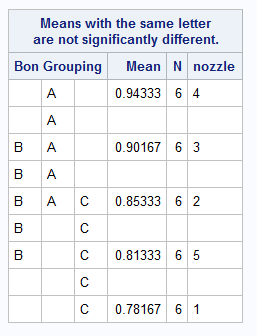
\includegraphics{prob4bon}

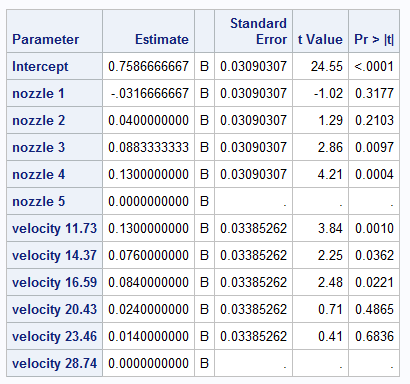
\includegraphics{PROB4EST}

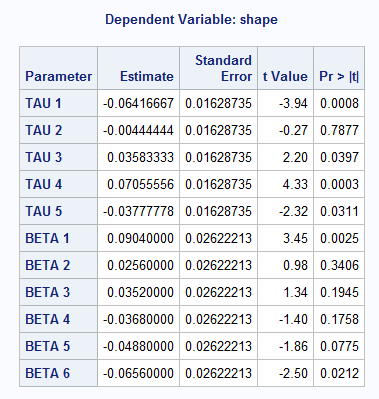
\includegraphics{prob4esttable}

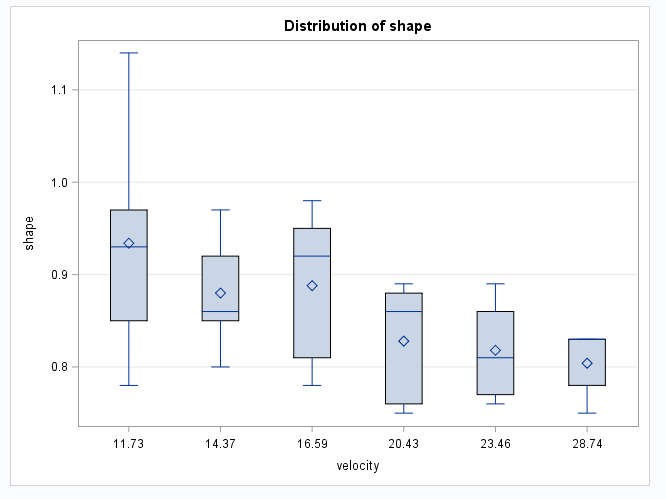
\includegraphics{prob4velocity}

\end{document}
